% ID: SEL-D0011-BA-E01
% ESTADO: validada. S012; tres pasadas del mismo autor, sin segundo revisor.
\textbf{Modelo de producción.}\par\nopagebreak[4]
Sean $x$ e $y$ las unidades por hora de los medicamentos A y B. Las condiciones y el beneficio por hora son
\[
\begin{cases}4\leq x+y\leq10,\\x-y\leq2,\\x\geq0,\quad y\geq0,\end{cases}
\qquad\max F(x,y)=60x+25y.
\]
La condición de política sanitaria significa $x\leq y+2$, no $x\leq2y$. Si se cuentan unidades completas, $x$ e $y$ son además enteros; veremos que el óptimo continuo ya lo es.

\textbf{Región factible y vértices.}\par\nopagebreak[4]
Intersecamos los semiplanos. En $x=0$ se obtiene $4\leq y\leq10$. Las fronteras $x-y=2$ y $x+y=4$ se cortan en $(3,1)$; con $x+y=10$ se obtiene $(6,4)$. No hay puntos factibles con $y=0$, pues exigirían a la vez $x\geq4$ y $x\leq2$. Los vértices, en orden, son
\[
\boxed{(0,4),\quad(3,1),\quad(6,4),\quad(0,10).}
\]
\begin{center}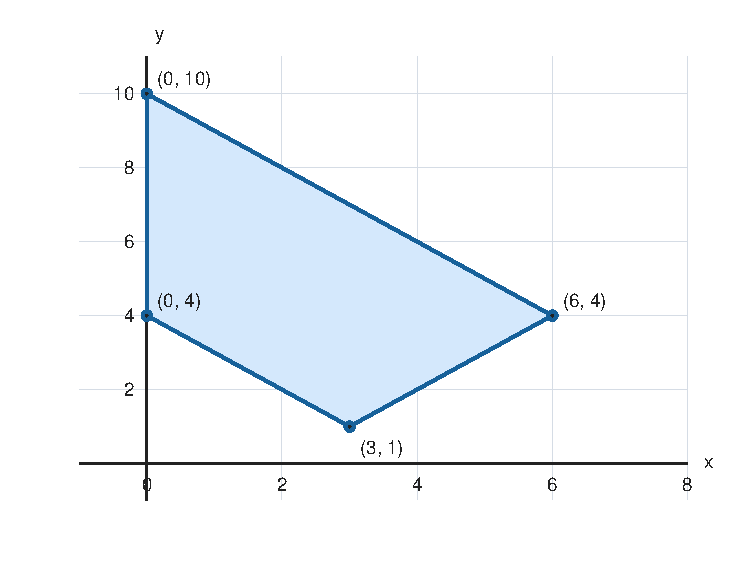
\includegraphics[width=0.51\linewidth]{recursos/figuras/s012-region.pdf}\end{center}

\textbf{Maximización y respuesta.}\par\nopagebreak[4]
Por ser lineal la función objetivo sobre un polígono compacto, basta evaluar los vértices:
\[
\begin{array}{c|rrrr}
(x,y)&(0,4)&(3,1)&(6,4)&(0,10)\\\hline
F\ (\text{euros/h})&100&205&460&250
\end{array}
\]
\boxed{6\text{ unidades A y }4\text{ unidades B por hora};\quad460\text{ euros/h}.}
El máximo es único. Se cumplen producción total $10$, diferencia $2$, no negatividad e integridad. Como comprobación global,
\[
F=42.5(x+y)+17.5(x-y)\leq42.5\cdot10+17.5\cdot2=460.
\]
La igualdad obliga a cumplir ambas fronteras con igualdad y determina precisamente $(6,4)$.
